%%%%%%%%%%%%%%%%%%%%%%%%%%%%%%%%
\chapter{Designing Native Restrictions}
%%%%%%%%%%%%%%%%%%%%%%%%%%%%%%%%
% State clearly definitions, assumptions, and proofs. The document will be archived for posterity and your name will be associated with any mistakes you make.
% Introduce and discuss the design decisions that you made during this project.
% Highlight why individual decisions are important and/or necessary. Discuss
% how the design fits together.
% Use as much as needed.

The goal is to port Java to native restrictions while applying a minimal set of changes to Java itself. We want Java to behave exactly like Native Image, and report missing registration errors for the exact same reasons that Native Image does. Our design targets \verb|labsjdk-ce-21|, a fork of OpenJDK 21. 
This section explains (1) how we model semantics changes through the concept of native restrictions, (2) how defining scopes in Java enables us to express these changes, and (3) how we improve Native Image usability.

%%%%%%%%%%%%%%%%%%%%%%%%%%%%%%%%
\section{Native Restrictions}
%%%%%%%%%%%%%%%%%%%%%%%%%%%%%%%%
We introduce the concept of language restrictions to model the set of semantics that Java runs with. These restrictions modify how dynamic class loading, dynamic invocation, and reflection behave at runtime. Each feature can be configured to either run under native restrictions and behave as in Native Image or to run without restrictions and behave like in Java.
At the two ends of the spectrum of the language restrictions, we have that when no restrictions are applied, Java behaves according to the Java Language Specification. When all the restrictions are applied, Java runs under native restrictions and behaves according to the Native Image Semantics, as presented in Section~\ref{native_image_specs}. 

The \emph{native restrictions checks} are runtime checks that we use to enforce native restrictions. They usually consist of a first check to see if the dynamic class loading, dynamic invocation, or reflection are running under native restrictions. If this is not the case, the check returns without side effects. Otherwise, additional operations can be applied, such as checking if an element is registered for reflection and throwing an exception if the semantics requires it. In doing so, we are effectively changing the behaviour of Java to match Native Image's.

%%%%%%%%%%%%%%%%%%%%%%%%%%%%%%%%
\section{Native Restrictions Scopes}
%%%%%%%%%%%%%%%%%%%%%%%%%%%%%%%%
To differentiate both runtime from build time behaviour and JVM calls from user calls, we use the notion of \emph{native restrictions scopes}. Opening a scope creates a region of code where Java is not constrained to native restrictions. 
More formally, let \verb|A| and \verb|C| be two classes or interfaces (in this thesis, the term class will refer to both classes and interfaces), let \verb|c| be a method of \verb|C|, and assume the existence of a mechanism to open scopes. As shown in Figure~\ref{fig:scopes}, \verb|c| opens a scope \verb|S|, invokes the method \verb|a| of \verb|A|, and closes \verb|S| when it returns from \verb|a|. Method \verb|a| invokes a method \verb|b|, which performs some native restriction checks.
Then if \verb|c| is invoked, the checks in \verb|b| will be ignored, as the invocation happened inside of the scope \verb|S|.
If the method \verb|a| or \verb|b| is invoked by another caller that does not open a scope, the native restrictions checks in \verb|b| will be enforced.

\begin{figure}[ht]
    \centering
\begin{lstlisting}[language=Java]
class A {
    public static void a() {
        b(); 
    }
    public static void b() {
        if (isFeatureRestricted() && !isScopeOpen()) {
            throw new MissingReflectionRegistrationError();
        }
    }
} 
class C {
    static void c() {
       ...
       try(NativeRestrictionsScope s = NativeRestrictionsScope.openScope()) {
            A.a();
       }
       ...
    }
}
\end{lstlisting}
    \caption{Inside the scope \texttt{s}, Java is not constrained to the native restrictions checks performed in \texttt{A.b()} and the \texttt{MissingReflectionRegistrationError} is not thrown. If the method \texttt{A.b()} is invoked from outside of a scope, then the checks will be enforced.}
    \label{fig:scopes}
\end{figure}

In the following subsections, we show in more detail how these scopes were chosen for dynamic class loading, dynamic invocation, and reflection and that they are correct according to Native Image's semantics.

%%%%%%%%%%%%%%%%%%%%%%%%%%%%%%%%
\subsection{Dynamic Class Loading}
%%%%%%%%%%%%%%%%%%%%%%%%%%%%%%%%
To simulate Native Image's behaviour for dynamic class loading, we require under native restrictions that defining a class at runtime with \verb|java.lang.ClassLoader#defineClass1|, \verb|java.lang.ClassLoader#defineClass2| or \verb|java.lang.ClassLoader#defineClass0| results in an \verb|UnsupportedOperationException|, unless the class is \emph{preloaded}. In Native Image, a class is preloaded if it is registered for reflection and has been linked at build time.
%Since the second clause cannot be reproduced in Java, we require the classpath.
Furthermore, a distinction between the initiator of the class loading must be made. The method \verb|java.lang.ClassLoader#loadClass| is the usual entry point to initiate class loading and can be invoked by the JVM internally or directly from user code. In the former case, we do not want an \verb|UnsupportedOperationException| to be thrown. In the latter case, we want to throw the exception if the class is not preloaded to prevent users from defining an arbitrary class at runtime.

We introduce the private wrapper method \verb|java.lang.ClassLoader#runtimeLoadClass| to differentiate the origin of the call that initiated class loading. Instead of directly calling \verb|loadClass|, the JVM now invokes the wrapper function, which dispatches the call to the delegate class loader, as intended when running without restrictions. As shown in Figure~\ref{fig:load_class}, the JVM is the only direct entry point to \verb|runtimeLoadClass|. When the JVM invokes the method, it opens a scope that closes on \verb|defineClass1|'s return. In this scope, class resolution proceeds as described in Background Section~\ref{dynamic_class_loading}. 
Directly calling \verb|loadClass|, on the other hand, does not open the scope and invoking \verb|defineClass1| will result in an \verb|UnsupportedOperationException|.

For the implementation of preloaded classes, we modify the method \verb|java.lang.ClassLoader#findLoadedClass|.
Under native restrictions, we check if the scope is open, in which case \verb|findLoadedClass| returns normally. If the scope is not open and the class is not registered for reflection a \verb|MissingReflectionRegistrationError| is thrown. If the class is registered, we simulate the class being preloaded by invoking \verb|Class#forName| with the application class loader and return the newly loaded class. Attempting to load a class that is not on the classpath will still result in an \verb|UnsupportedOperationException|.

% If not preloaded, then a class may be defined at runtime only if resolving the class or interface was required by one of the following instructions:
% anewarray, checkcast, getfield, getstatic, instanceof, invokedynamic, invokeinterface, invokespecial,
% invokestatic, invokevirtual, ldc, ldc\_w, multianewarray, new, putfield, and putstatic.

\begin{figure}
    \centering
    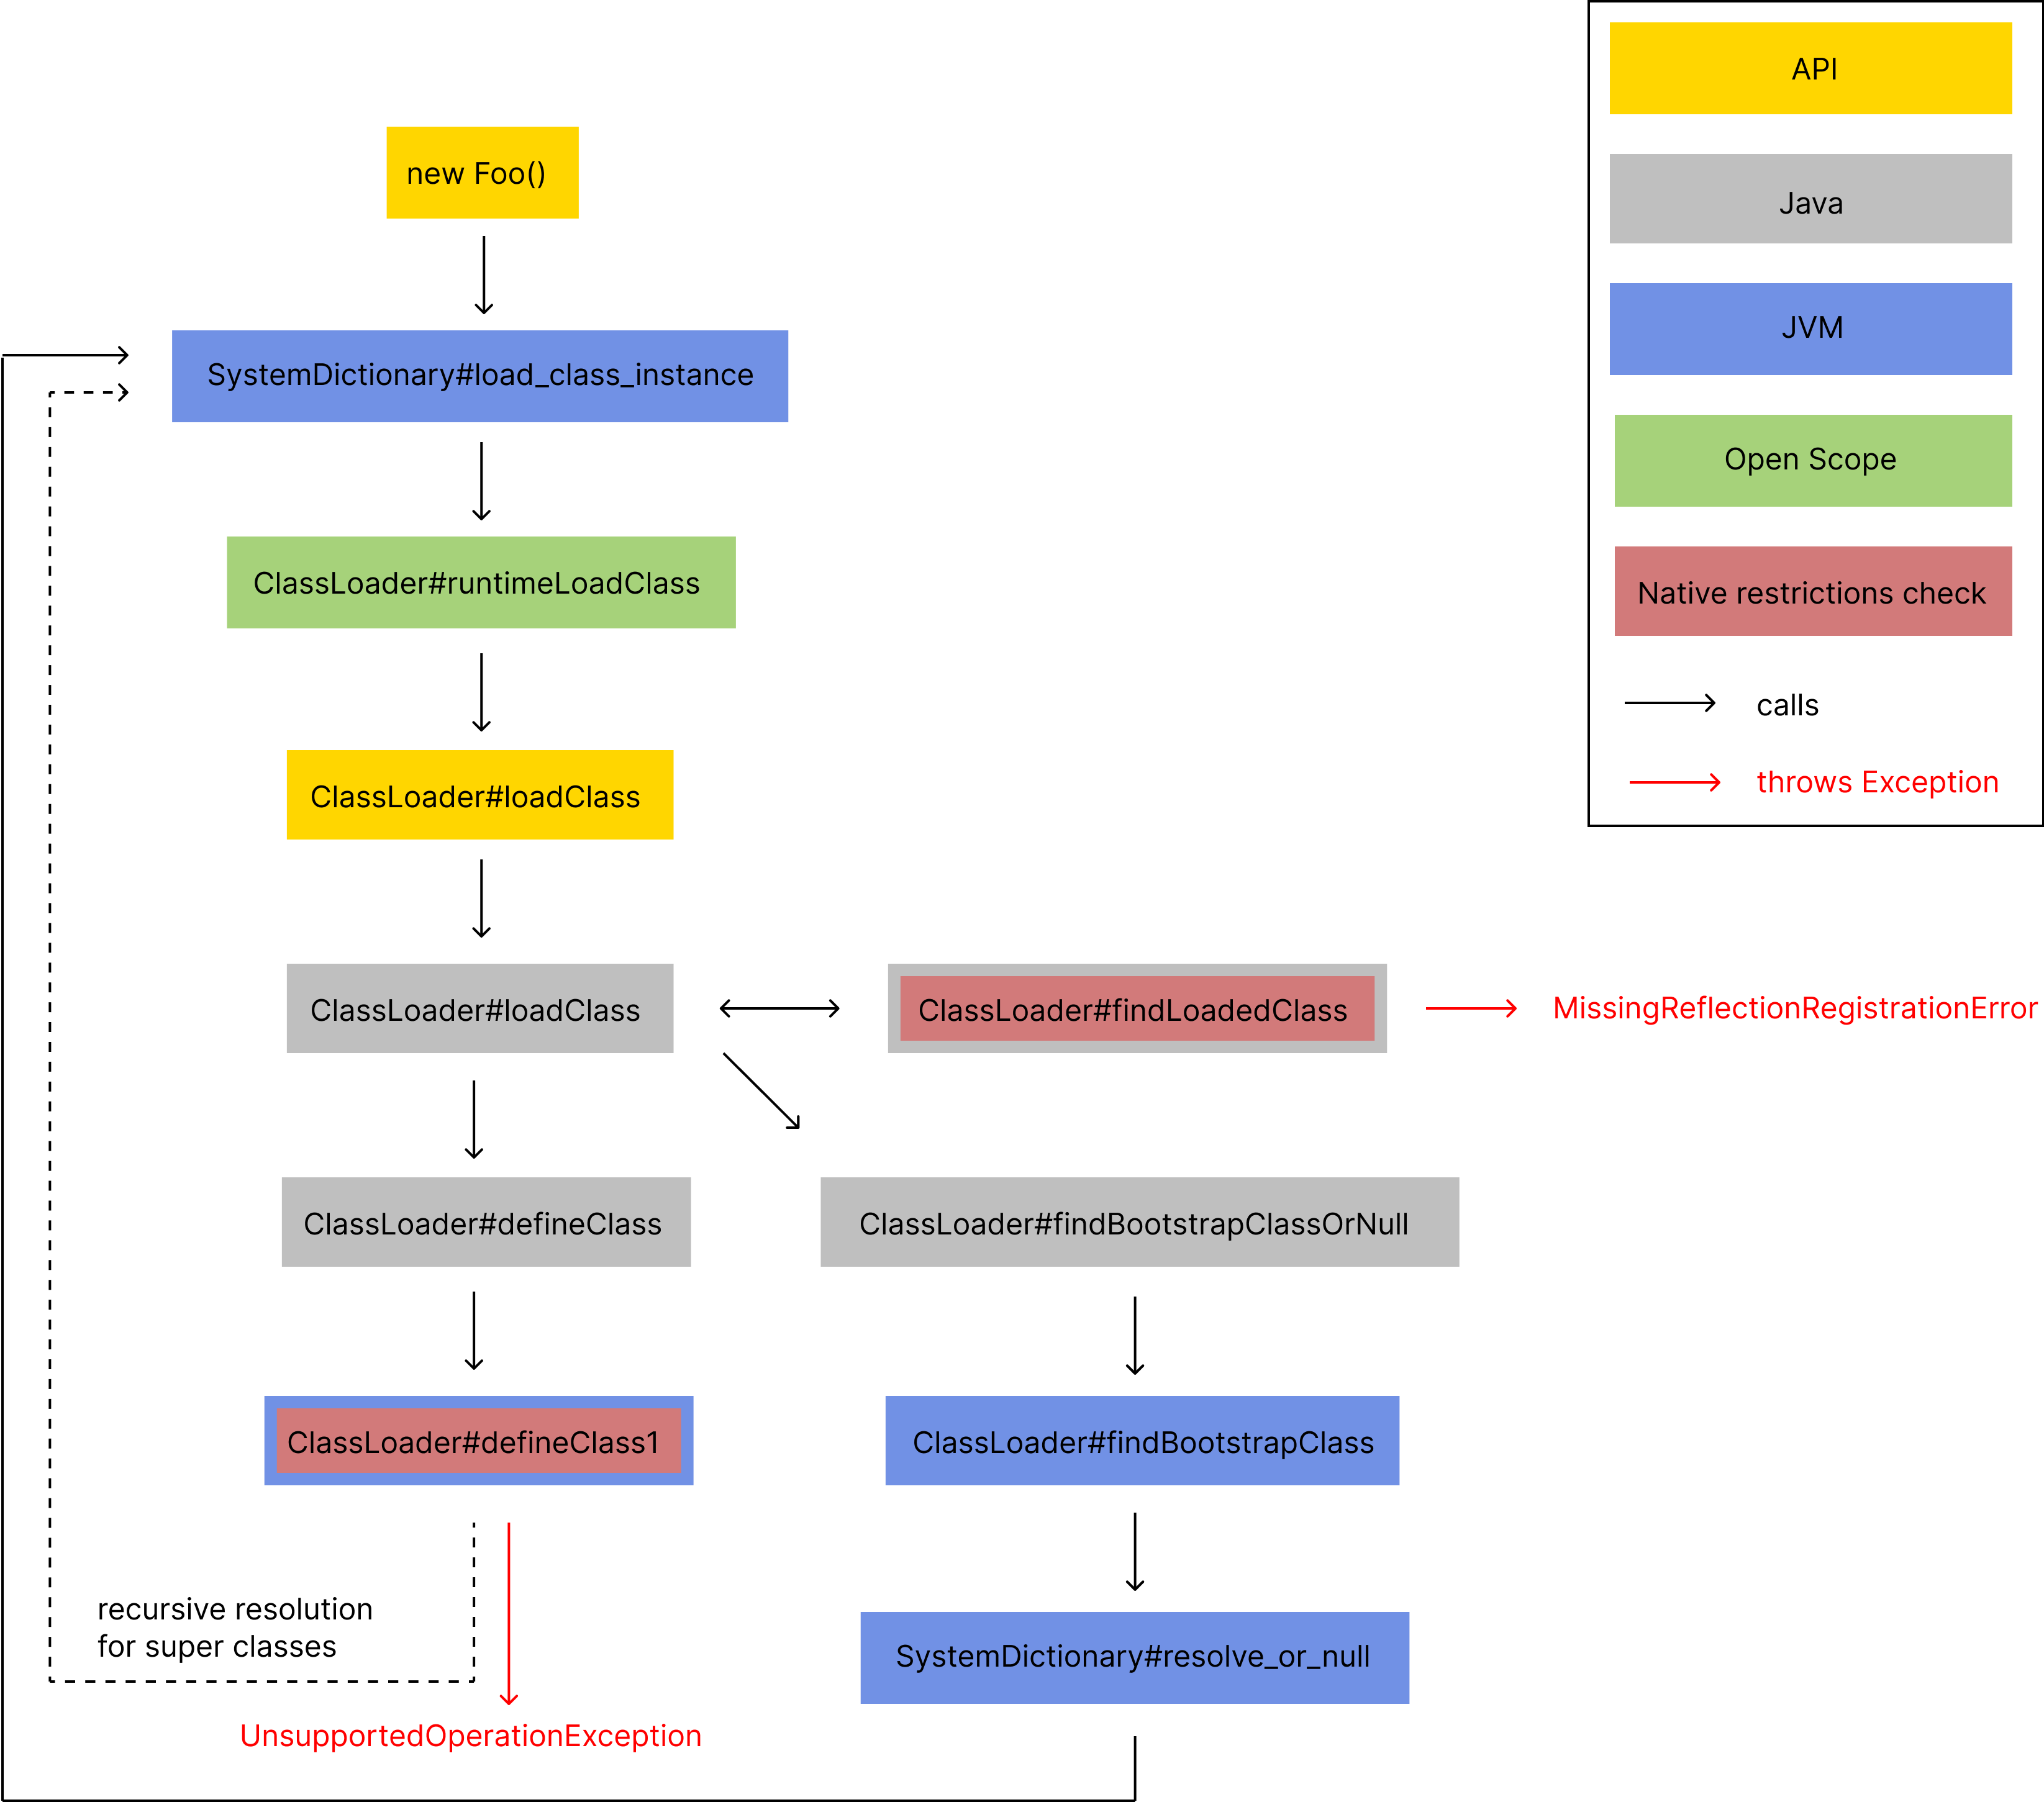
\includegraphics[scale=0.5]{resources/Group 412.png}
    \caption{Calling sequence for class loading, with the wrapper function \texttt{runtimeLoadClass} and scopes to support dynamic class loading at runtime.}
    \label{fig:load_class}
\end{figure}

The design of dynamic invocation under native restrictions required multiple iterations to keep the changes to a minimum. Figure~\ref{fig:define_class_0} shows all the entry points from which \verb|java.lang.ClassLoader#defineClass0| can be invoked to define a hidden class as part of the of the dynamic invocation process and illustrates the final state of the design. 

Under native restrictions the methods \verb|metafactory| and \verb|altMetafactory| of \verb|java.lang.invoke.LambdaMetfactory| throw an \verb|UnsupportedOperationException| to prevent the execution of arbitrary code at runtime, unless the invocation is part of the \verb|invokedynamic| instruction.
To differentiate both behaviours, we open a scope in \verb|java.lang.BootstrapMethodInvoker#invoke|. The method is invoked by the JVM in the process of linking the \verb|CallSite|, when resolving the bootstrap method. Following Native Image's semantics, the scope is opened if and only if Native Image also compiles this bootstrap method at build time. Figure~\ref{fig:define_class_0}, shows that moving the opening of the scope up or down on the stack trace would introduce an additional change because of the branching out. We also do not have the required metadata on the bootstrap method to place it in the JVM.

% Certain user calls can trigger the definition of internal Java classes at runtime, for performance reason we treat these calls differently in Java under native restrictions.
Specific user calls can trigger the definition of internal Java classes at runtime; for performance reasons, we treat these calls differently in Java under native restrictions.
Concretely, the invocation or binding of a method handle and the lookup of an executable or field can result in the resolution of a method handle such that the JVM emits instructions to define internal classes of Java at runtime. During the resolution process, the JVM can, as an optimization, compile internal classes, such as a \verb|java.lang.invoke.LambdaForm| and specialized form of \verb|BoundMethodHandle|.
In Native Image, these hidden classes are forced-interpreted, and method handles are resolved through reflection. As such, letting Java under native restrictions define these classes and defer the restrictions checks to the resolution of method handle, as seen in the next section, does not contradict the semantics of Native Image. Therefore, for performance reasons, we opt to open scopes in \verb|jdk.internal.reflect.MethodAccessGenerator#invoke|, and in the methods \verb|InvokeBytecodeGenerator#loadMethod|, \verb|MethodHandle.BindCaller#makeInjectedInvoker|, and \verb|ClassSpecializer#loadSpecies| of the \verb|java.lang.invoke| package. These changes correspond to the top part of the stack traces on the graph of Figure~\ref{fig:define_class_0}. By the same process as the \verb|LambdaMetfactory|, and because none of the paths that need to implement native restrictions checks systematically meet at a node, we can prove that moving any of the scopes up or down on the stack trace would lead to the same amount or strictly more modifications.

\begin{figure}
    \centering
    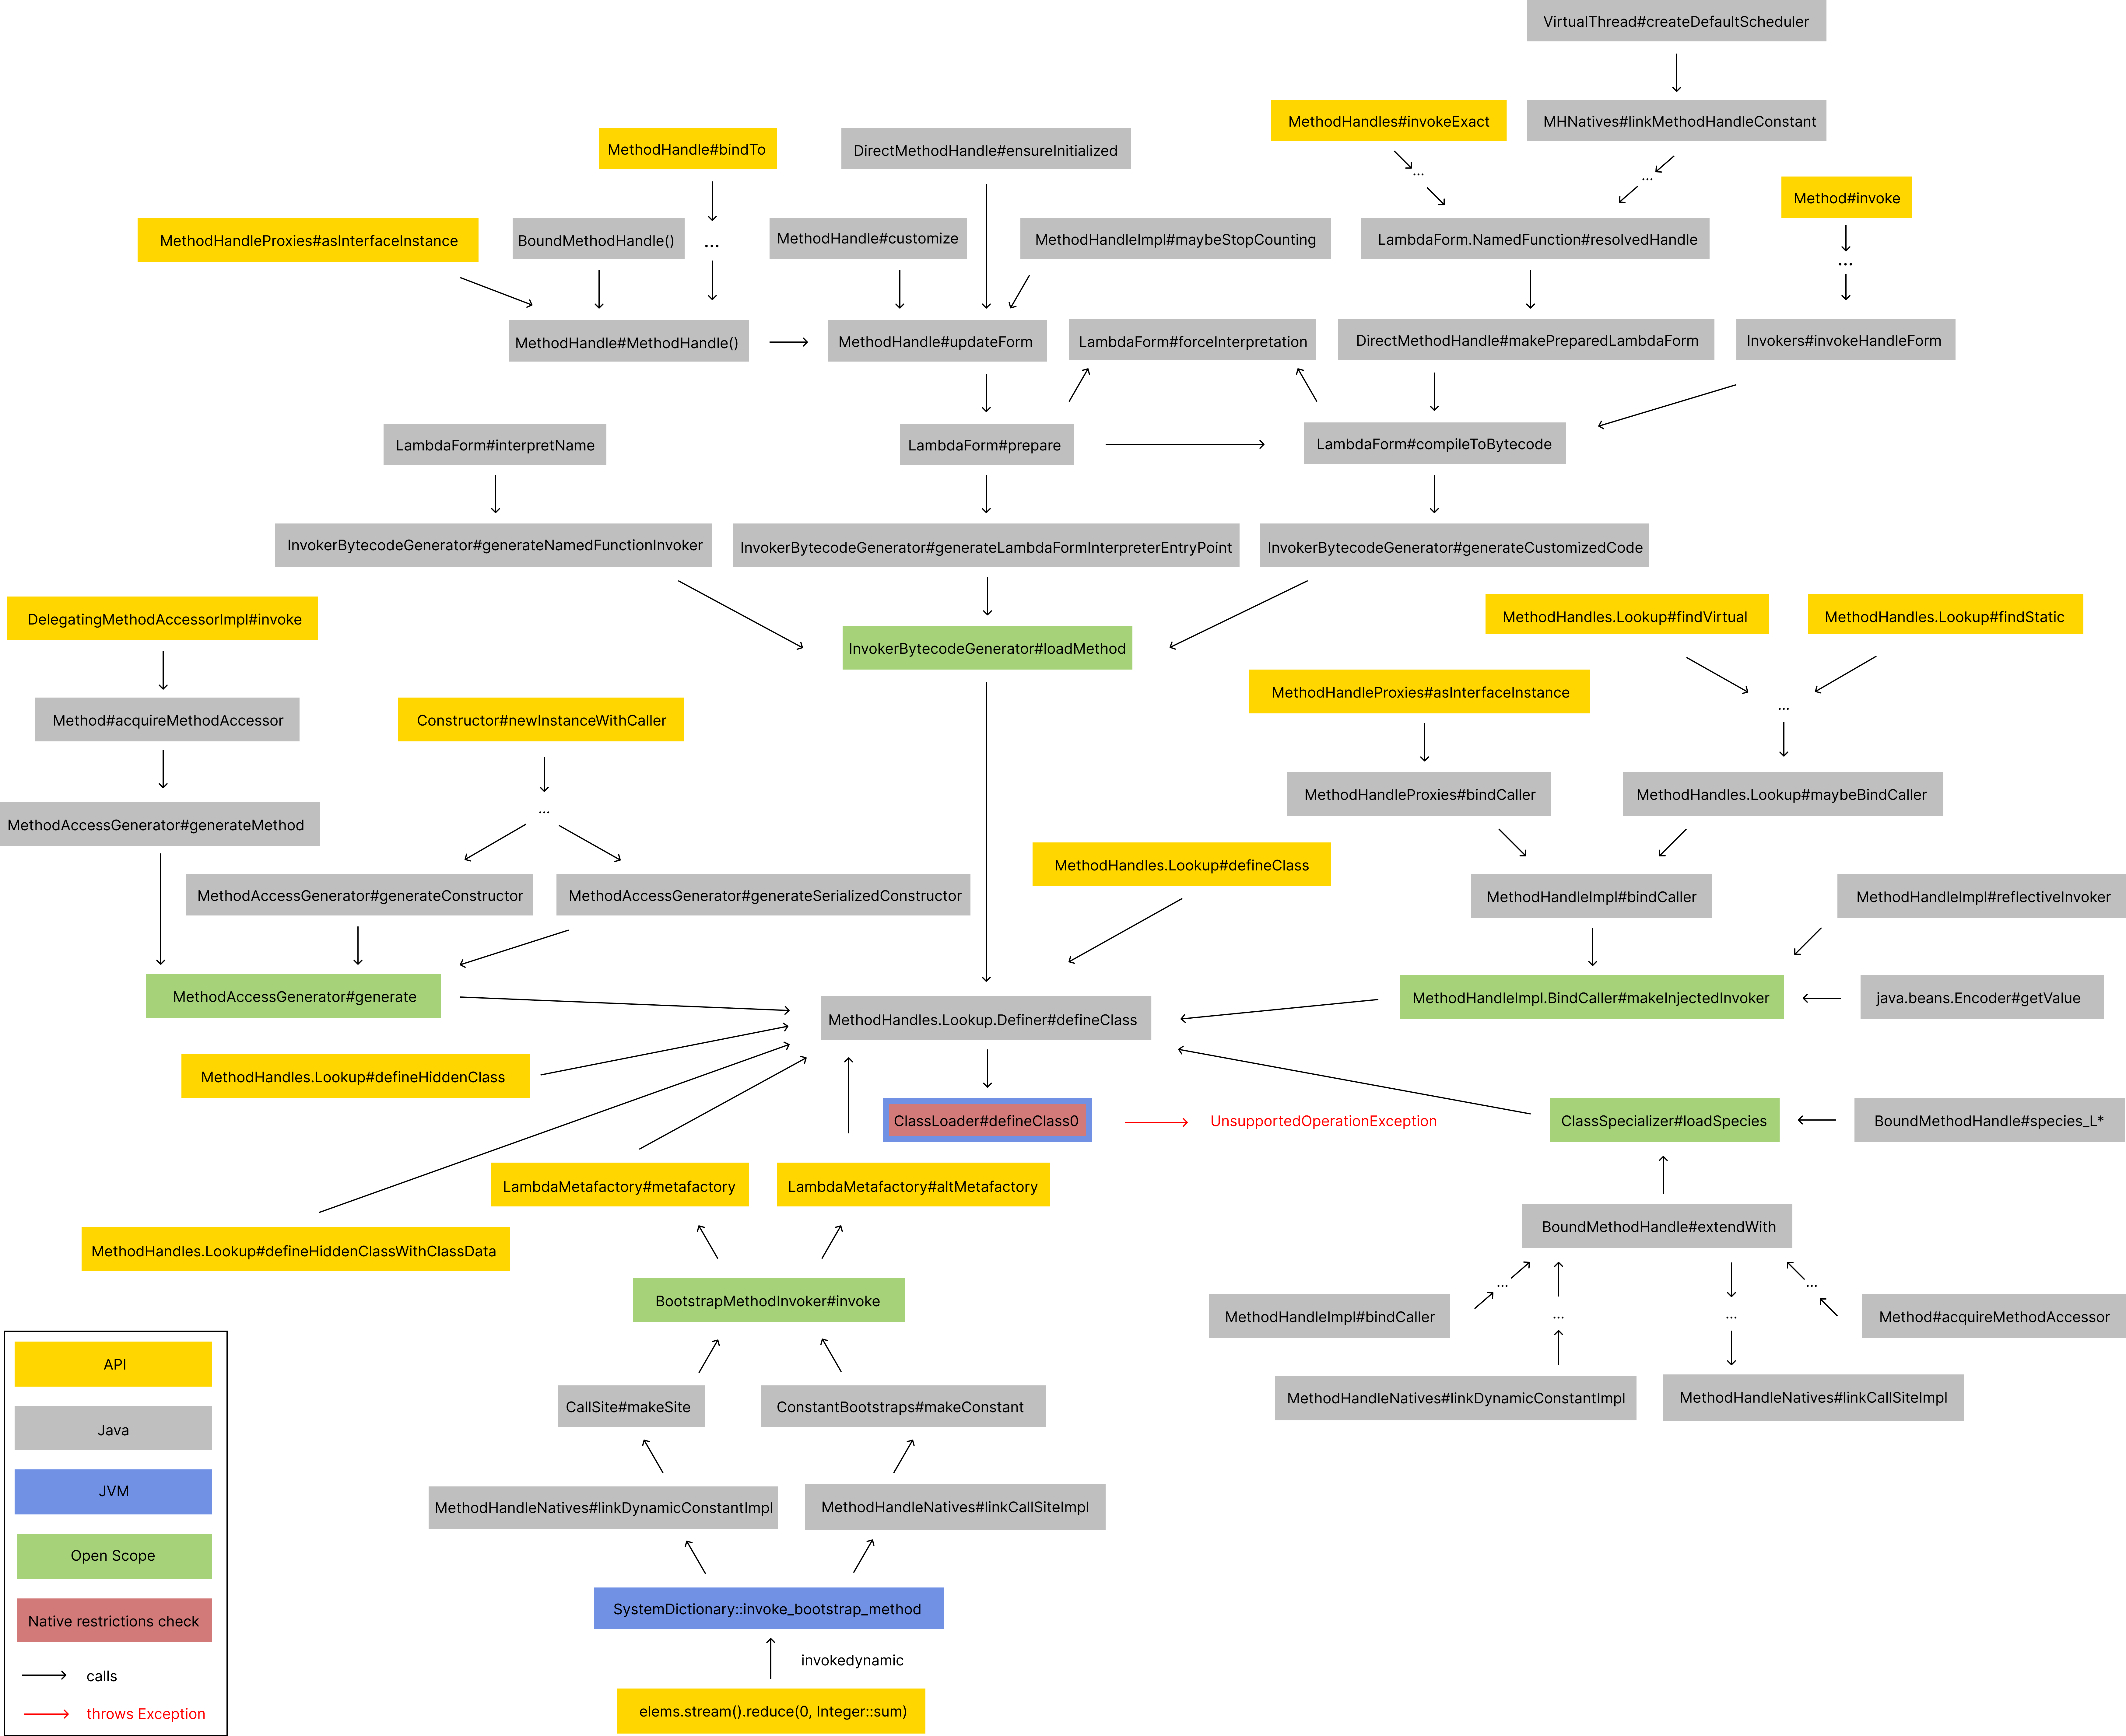
\includegraphics[angle=90,origin=c,scale=0.35]{resources/Group 413.png}
    \caption{Entry points for the method \texttt{java.lang.ClassLoader\#defineClass0}. For readability, the stack trace is not exhaustive and focuses on methods that have multiple callers.}
    \label{fig:define_class_0}
\end{figure}


Since the Java Native Interface~(JNI)~\cite{noauthor_jni_nodate} allows users to make downcalls to the JVM's implementation of the methods \verb|defineClass1|, \verb|defineClass2|, and \verb|defineClass0|, the native restriction checks must be placed in the JVM rather than in Java. We insert the checks in the JVM's method \verb|SystemDictionary::resolve_from_stream|, which is part of the common code for \verb|JVM_DefineClass| and \verb|JVM_DefineClassWithSource|. If none of the scopes are open, the call will result in an \verb|UnsupportedOperationException|. 

Through a static study of entry points and stack traces and the introduction of a few native restrictions scopes, we prove that the semantics of Java for dynamic class loading can be changed such that it simulates Native Image's.

%%%%%%%%%%%%%%%%%%%%%%%%%%%%%%%%
\subsection{Reflection}
%%%%%%%%%%%%%%%%%%%%%%%%%%%%%%%%
Modifying the reflection feature under native restrictions consists in adding native restrictions checks to all methods in the class \verb|java.lang.Class|, the package \verb|java.lang.invoke.reflect|, and \verb|jdk.internal.sun.misc.Unsafe|, that returns a reflectively-accessed element. Section~\ref{native_image_specs} describes the list of checks in more detail. 
If the element is not registered for reflection, a \verb|MissingReflectionRegistrationError| is thrown.
To check if an element is registered, we load all JSON reflection configuration files that are on the classpath or user-defined. The classes and interfaces to parse the JSON reflection configuration file and the data structure that holds the configuration are taken directly from Native Image. Changes made to that part of the code in Native Image can be easily adapted to work in Java under native restrictions.

In Java under native restrictions we modify the process of \verb|MethodHandle| resolution to match Native Image's semantics.
The resolution of a method handle can occur, from the user perspective, either as the result of the dynamic invocation of a method or as the result of a lookup.
Similarly to reflection, \verb|java.lang.MethodHandles.Lookup| provides an API to look up \verb|Executables|, \verb|Fields|, and \verb|VarHandles|, and returns a method handle to access the element. 
In Native Image, the \verb|MemberName| encapsulated in the method handle is resolved through reflection if it does not reference an intrinsic method. To simulate this behaviour in Java under native restrictions, we introduce a native restriction check in the \verb|java.lang.invoke.MemberName#resolve|. 
For intrinsic methods, we keep a hard-coded list of \verb|MemberName| that do not require reflection to be resolved. Scopes cannot be used in this case, as invoking any method to open a scope relies on these same intrinsic method handles.
Moreover, as parts of the internal code for reflection configuration use lambda expressions, we also open a scope in \verb|MethodHandles#linkMethodHandleConstant| to prevent cyclic dependencies.

During reachability analysis, Native Image can prove that internal classes accessed reflectively from the Java language to the Java language are reachable and do not need to be specified in the metadata. 
%Internally, the JVM uses reflection to access internal Classes, Executables and Fields. 
To invoke a method obtained via a lookup, for example, the JVM will reflectively access the method \verb|java.lang.invoke.MethodHandle#invokeBasic|. Because Native Image can prove from the code that these elements are reachable, these calls from the JVM to the JVM are not constrained to native restrictions. To filter out these accesses, Java under native restrictions implements an \verb|AccessAdvisor|, adapted from the \verb|AccessAdvisor| used by GraalVM's Tracing Agent. The advisor contains a list of classes and patterns (e.g., \verb|java.lang.**|), such that if the caller at the origin of the reflective access is included in that list, the native restrictions checks are ignored.

Building on top of Java under native restrictions for dynamic class loading, we add native restrictions checks to verify that every reflectively-accessed element is registered for reflection and we introduce an \verb|AccessAdvisor| to filter out calls from the JVM to the JVM that can safely be ignored.

%%%%%%%%%%%%%%%%%%%%%%%%%%%%%%%%
\section{Improving Usability}
%%%%%%%%%%%%%%%%%%%%%%%%%%%%%%%%
In this section, we will see how Java under native restrictions fits in the overall Native Image usability plan by improving the turnaround for computing reachability metadata and defining the expected behaviour of Native Image. 

%%%%%%%%%%%%%%%%%%%%%%%%%%%%%%%%
\subsection{Streamlining reachability metadata computation}
%%%%%%%%%%%%%%%%%%%%%%%%%%%%%%%%
One of the primary goals of this thesis is to streamline reachability metadata computation for users.
The first step in the computation of the metadata is the collection. To achieve this, GraalVM's Tracing Agent automatically collects the reachability metadata required for an application. The issue with the current implementation is that the JVM to which it is attached does not follow Native Image's semantics. As a result, the agent can take an entirely different path during execution than Native Image, and miss reflectively-accessed elements. Moreover, attaching an agent to the JVM significantly slows down the execution.
Our solution to this problem is to implement another Tracing Agent in Java. The Tracing Agent is another language restriction designed to follow the exact same path during an execution as Java under native restrictions. Instead of performing restriction checks, the agent logs the reflectively-accessed elements and outputs a JSON reflection configuration at the end of the execution run. 
Once the metadata are collected, the configuration can be tested on Java under native restrictions, thus avoiding the overhead of building an image. The Evaluation Section~\ref{benchmark} illustrates that this overhead is non-negligible when it comes to testing.  

We propose a new and optimized workflow for computing metadata: (1) run the agent, (2) test the JSON reflection configuration with Java under native restrictions, (3.a) if the execution did not result in an exception, build the image, (3.b) otherwise debug the application by attaching a Java debugger to Java under native restrictions if needed.

%%%%%%%%%%%%%%%%%%%%%%%%%%%%%%%%
\subsection{Defining expected behaviour}
%%%%%%%%%%%%%%%%%%%%%%%%%%%%%%%%
The Technology Compatibility Kit~(TCK) is our first approach to specifying the semantics of Native Image for dynamic class loading and reflection. The TCK is a test suite that illustrates the specifications. It gives concrete examples of the expected behaviours and provides a future-proof way of asserting that different versions of Native Image still behave according to the same semantics.
It is designed to run with both Native Image and Java under native restrictions.

Test harnesses usually rely on annotations to get the test classes and individual tests to run, but using reflection in the TCK to test reflection is not an option. JUnit's~\cite{noauthor_junit_nodate} \verb|@Test| annotation on methods, for example, can be reflectively queried to obtain the test \verb|Method| to invoke in the test harness. Instead, we rely on an annotation processor to generate on the fly all the data structure needed to run the test harness at compile time without using any reflective call (see Section~\ref{TCK} for details on the implementation).

The TCK contains positive and negative unit tests for dynamic class loading and reflection. To guarantee the correctness of the tests themselves, in particular for reflection, each test uses reflection on different dummy classes, so that the tests do not interfere with each other.
The test uses the \verb|opaque| method, as seen in Figure~\ref{fig:opaque}, to wrap arguments passed for reflection and ensure that no compiler optimization is done across the call.

\begin{figure}[ht]
    \centering
\begin{lstlisting}[language=Java]
public static <T> T opaque(T value) {
    System.out.printf("");
    return value;
}
\end{lstlisting}
    \caption{The \texttt{opaque} method does nothing but ensures that the provided argument does not get constant-folded by the compiler.}
    \label{fig:opaque}
\end{figure}

Despite - or thanks to - its simplicity, the TCK did enable us to catch bugs in Native Image. Some of the bugs, as seen in Figure~\ref{fig:new_multi_array_bug}, are easy to fix, as Native Image only returns the wrong type of exception.  
Instantiating a new array is supported in Native Image if the component type of the array is registered for reflection. However, currently, trying to instantiate a new array without registering \texttt{C} for reflection throws a fatal error \texttt{java.lang.IllegalArgumentException} that cannot be caught instead of throwing a \verb|MissingReflectionRegistrationError|. Similarly, trying to instantiate a new multi-dimension array without registering \texttt{C} for reflection throws a \texttt{com.oracle.svm.core.jdk.UnsupportedFeatureError}, even though the feature is supported and only requires the class to be registered to work.

\begin{figure}[ht]
    \centering
\begin{lstlisting}[language=Java]
class C {
}

class Main {
    public static void main(String[] args) throws Exception {
        Array.newInstance(opaque(C.class), 5);
        Array.newInstance(opaque(C.class), 5, 5);
    }
}
\end{lstlisting}
    \caption{Example of bug caught with the TCK where Native Image's behaviour deviated from the expected behaviour.}
    \label{fig:new_multi_array_bug}
\end{figure}

We found another bug with the TCK, which concerned the registration of superclasses. For a class \verb|B| that extends \verb|A|, if \verb|B| is registered for reflection but \verb|A| is not, then invoking \verb|Class#forName(opaque("A"))| still returns the class without throwing an exception, which is wrong according to Native Image's semantics. 
We also found a performance bug for a preview feature of Java 21. The \verb|java.util.FormatProcessor| uses a bootstrap method that Native Image currently interprets. Over 100'000 iterations, running the program shown in Listing ~\ref{fig:format_processor} with Native Image is 2X slower than with HotSpot. This bootstrap method can be proven safe to compile at build time, and the overhead of interpreting it at runtime could be avoided. By compiling the method, we can obtain a speedup of 3X compared to HotSpot.

\begin{figure}[ht]
    \centering
\begin{lstlisting}[language=Java]
public class Main {
    public static void main(String[] args) {
        String str = FormatProcessor.FMT."Hello there!";
    }
}
\end{lstlisting}
    \caption{The \texttt{FormatProcessor} uses the bootstrap method \texttt{java.lang.runtime.TemplateRuntime.processStringTemplate}, which can be proven safe to compile at build time. }
    \label{fig:format_processor}
\end{figure}

The TCK provides a representation of Native Image's semantics and proves that with a few unit tests and a clear semantics, we can already improve Native Image usability by detecting unexpected behaviours.
% Balance between what needs to be changed in Native Image, driving the specs with this Java mode, and using part of what is in Nativ eImage in Java mode (e.g. 
% MissingReflectionRegistrationError is still in progress in Native Image, but also using in Java).

% Building the agent after doing the defineClass -> back and forth
% SecurityManager was changed in Java moide, so had to change in NI, but other changes were made in NI so also had to propagate back the changes into the Java mode.
% etc.

%%%%%%%%%%%%%%%%%%%%%%%%%%%%%%%%
\chapter{Implementation}
%%%%%%%%%%%%%%%%%%%%%%%%%%%%%%%%
% The implementation covers some of the implementation details of your project.
% This is not intended to be a low level description of every line of code that
% you wrote but covers the implementation aspects of the projects.
% Please provide as stable as possible links to the implementation source code.

This section discusses implementation details of the native restrictions, the scopes and checks, and the TCK.

%%%%%%%%%%%%%%%%%%%%%%%%%%%%%%%%
\section{LanguageRestrictionManager}
%%%%%%%%%%%%%%%%%%%%%%%%%%%%%%%%
The \verb|LanguageRestrictionManager| is the main entry point to the language restrictions. It provides a singleton instance of the abstract class \verb|LanguageRestriction|, which is the superclass of: 
\begin{itemize}
    \item \texttt{NativeLanguageRestriction} which models Native Image semantics
    \item \texttt{NoLanguageRestriction} which  models Java semantics
    \item \texttt{NativetraceLanguageRestriction} for the Java Tracing Agent that we implemented
\end{itemize}
The type of \verb|LanguageRestriction| is selected by setting the System property \verb|language.restriction| to either \verb|'native'|, \verb|'none'| or \verb|'native-trace'|. 

The \verb|LanguageRestrictionManager| is the interface for every native restrictions checks, and is used to hide away the scope abstraction when possible.
The language restriction is initialized during the last phase of the VM initialization and loads the reflection configuration.
% object into an instance of \verb|TypeConfiguration|, 
%%%%%%%%%%%%%%%%%%%%%%%%%%%%%%%%
\section{Native Restrictions Scopes}
%%%%%%%%%%%%%%%%%%%%%%%%%%%%%%%%
We implemented native restrictions scopes with thread local counters. Using thread locals prevents the opening of a scope on one thread from interfering with another thread's scopes.
Concretely, each time a scope is opened, the counter is incremented, and each time a scope is closed, the counter is decremented. The counter also accounts for recursive calls: the scope is either open or closed until the base case of the recursion returns.
To avoid memory leaks, the thread local is instantiated in a \verb|try-with-resource| block statement (see Figure~\ref{fig:bind_caller_twr}) and implements the \verb|AutoCloseable| interface, which calls the method \verb|close| to release resources on return or when an exception occurs.

\begin{figure}[ht]
    \centering
\begin{lstlisting}[language=Java]
static MethodHandle bindCaller(MethodHandle mh, Class<?> hostClass) {
    try (NativeRestrictions unused = NativeRestrictions.openScope()) {
        return BindCaller.bindCaller(mh, hostClass);
    }
}
\end{lstlisting}
    \caption{Explicit try-with resource block statement to open a scope in Java under native restrictions.}
    \label{fig:bind_caller_twr}
\end{figure}

As seen in Figures~\ref{fig:bind_caller_lambda} and~\ref{fig:bind_caller_lrm}, to minimize the changes made to Java, the \verb|try-with-resource| block statement is hidden in the \verb|LanguageRestrictionManager| and the region of code that was in the block in Figure~\ref{fig:bind_caller_twr} is passed as a lambda expression and invoked in the \verb|LanguageRestrictionManager|. Hiding the scope opening in a lambda is only possible for a region of code that is not on the path of an \verb|invokedynamic| instruction, as this would create a cyclic dependency. 

\begin{figure}[ht]
    \centering
\begin{lstlisting}[language=Java]
static MethodHandle bindCaller(MethodHandle mh, Class<?> hostClass) {
    return LanguageRestrictionManager.bindCallerCheck(() -> 
        BindCaller.bindCaller(mh, hostClass));
}
\end{lstlisting}
    \caption{Lambda expressions are used to hide implementation details in the \texttt{LanguageRestrictionManager} and minimize changes made to the JDK.}
    \label{fig:bind_caller_lambda}
\end{figure}

\begin{figure}[ht]
    \centering
\begin{lstlisting}[language=Java]
public static MethodHandle bindCallerCheck(Supplier<MethodHandle> s) {
    try (NativeRestrictions unused = NativeRestrictions.openScope()) {
        return s.get();
    }
}
\end{lstlisting}
    \caption{Implementation of the native restrictions checks in the \texttt{LanguageRestrictionManager} when the supplier \texttt{s} is passed as a lambda expression from the JDK.}
    \label{fig:bind_caller_lrm}
\end{figure}

%%%%%%%%%%%%%%%%%%%%%%%%%%%%%%%%
\section{Technology Compatibility Kit}\label{TCK}
%%%%%%%%%%%%%%%%%%%%%%%%%%%%%%%%
The TCK is a test suite for Native Image and Java under native restrictions that tests Java's dynamic features and reflection. 
%As the test harness cannot rely on reflection, we use an annotation processor to generate all the data structures needed to invoke the tests. 
It is Gradle~\cite{noauthor_gradle_2024} project composed of 4 sub-projects: 
\begin{itemize}
    \item the \verb|annotation-processor| contains all the logic for the annotation processor and the generation of scripts to run the TCK
    \item the \verb|tck| contains the tests classes
    \item the \verb|tck-harness| contains the test harness to run the test and asserts the results
    \item the \verb|tck-utils| contains common utility classes
\end{itemize}
The separation of the features into sub-projects simplify the compilation chains, as the first three sub-projects depend on the \verb|tck-utils|, the \verb|tck| depends on the \verb|annotation-processor|, and the \verb|tck-harness| depends on the \verb|tck|.

The TCK aims to assert that Native Image and Java under native restrictions follow the correct semantics. Therefore, it must also be able to run tests both with and without reachability metadata. Since, by default, all tests in a test class share the same metadata and are built into a single image for Native Image, a second requirement is that a test should be able to run in isolation and have its own separate image and metadata. 
Figure~\ref{fig:tck_for_name} is an example of a test that the TCK can run. Each test in the suite is annotated with the \verb|@Test| annotation. The annotation contains fields for the reflection metadata, for the expected exception when the test runs without the metadata, and an optional field \verb|sinceVersion|, if a previous version of Native Image did not behave as expected. The \verb|@NativeImageTCKDeviation| means that the current version of Native Image does not return the expected behaviour. Finally, \verb|@RunTestInIsolation| can be used to run the test in an isolated image. 

\begin{figure}[ht]
    \centering
\begin{lstlisting}[language=Java]
@Test(
    reflectionMetadata =
            """
            [{
                "name": "ForNameTestClass"
            }]
            """,
    expectedNoRegistrationException = MISSING_REFLECTION_REGISTRATION_ERROR
)
@RunInIsolation
@NativeImageTCKDeviation(ticketNumber = "GR-123456")
public static void forName() throws Exception {
    Class<?> result = Class.forName(opaque("ForNameTestClass"));
    assertEquals(opaque(ForNameTestClass.class), result);
}
\end{lstlisting}
    \caption{Example of a test that expects a \texttt{ForNameTestClass.class} to be returned when the class is registered and a \texttt{MissingReflectionRegistrationError} to be thrown otherwise. It runs in its own \texttt{native-image} and the issue \texttt{GR-123456} has been filed because Native Image does not currently behave as expected.}
    \label{fig:tck_for_name}
\end{figure}

To implement these features, the annotation processor does most of the heavy lifting. The annotation parsing phase is made of three steps:
\begin{enumerate}
    \item It maps each test class to a list of \verb|TestData| Records 
    \item It parses the \verb|reflectionMetadata| field of each test and generates the associated JSON reflection configuration in a \verb|reflect-config.json| files
    \item It generates bash scripts for Native Image and Java with the command to run the test harness with and without metadata for each test class and isolated test
\end{enumerate}
The \verb|TestData| contains, for each test, the expected results when running without registration, an optional \verb|sinceVersion|, a boolean for if it should run in isolation and if Native Image's behaviour deviates, and a \verb|Callable|, such that the test harness can invoke the method without relying on reflection.  
A \verb|TestRunnerMap.java| file is automatically generated during the annotation parsing, and contains the map described in 1., with its entry statically initialized. 

To run the tests in the TCK, the test harness instantiates an instance of \verb|TestRunnerMap| at runtime, iterates through the entries, invokes the \verb|Callable| in the \verb|TestData|, and asserts that the returned result is correct.

%%%%%%%%%%%%%%%%%%%%%%%%%%%%%%%%
% \section{Dynamic Class Loading}
%%%%%%%%%%%%%%%%%%%%%%%%%%%%%%%%
% Native Image does not allow for runtime definition of classes that were not preloaded beforehand.
% To simulate this behaviour, we introduce the wrapper method java.lang.ClassLoader#runtimeLoadClass. The only entry point for this private method is the interpreter. If not preloaded, then a class may be defined at runtime only if resolving the class or interface was required by one of the following instructions:
% anewarray, checkcast, getfield, getstatic, instanceof, invokedynamic, invokeinterface, invokespecial,
% invokestatic, invokevirtual, ldc, ldc\_w, multianewarray, new, putfield, and putstatic.
% The wrapper then dispatches the call to the method loadClass to the delegate class loader, as intended when running without restrictions.
% Runtime calls to the public method java.lang.ClassLoader#loadClass methods first checks if the class was preloaded (i.e. checking the inclusion of the class in the reflection metadata is sufficient to simulate Native Image behaviour in this Java mode), before allowing it to be defined.

%%%%%%%%%%%%%%%%%%%%%%%%%%%%%%%%
\chapter{The Native Image Reflection Semantics}\label{native_image_specs}
%%%%%%%%%%%%%%%%%%%%%%%%%%%%%%%%


%% TODO add snippets of code to show how it differes from normal Java

% ## Unimplemented Features
% #### java.lang.SecurityManager
% The `java.lang.SecurityManager` behaves in the following ways:
% * `java.lang.System#getSecurityManager()` always returns `null`
% * `java.lang.System#setSecurityManager(SecurityManager sm)` returns without exception if `sm` is null. 
% It throws a `SecurityException` if the system property `java.security.manager` is not set to `disallow`, and an 
% `UnsupportedOperationException` otherwise.


%%%%%%%%%%%%%%%%%%%%%%%%%%%%%%%%
\chapter{Evaluation}
%%%%%%%%%%%%%%%%%%%%%%%%%%%%%%%%
% In the evaluation you convince the reader that your design works as intended.
% Describe the evaluation setup, the designed experiments, and how the
% experiments showcase the individual points you want to prove.
In this section we show that the design of Java under native restrictions is correct according to Native Image's semantics and that it allows for visible improvements when it comes to testing the reachability metadata configuration.

%%%%%%%%%%%%%%%%%%%%%%%%%%%%%%%%
\section{Correctness of Java under native restrictions}
%%%%%%%%%%%%%%%%%%%%%%%%%%%%%%%%
To verify that Java under native restrictions is indeed correct with regard to the semantics of Native Image, we run the TCK with and without the reachability metadata and assert that our implementation does throw an exception in the correct place when the metadata is missing and returns the expected results otherwise. This evaluation step trivially succeeded, as the development of Java under native restrictions was partly test-driven by the TCK.

The other way of asserting the correctness of our implementation is with the JCK. The JCK is a proprietary test suite from Oracle that is used used to assert that a Java implementation complies with the Java Language Specification. A CI job is available on the enterprise repository to run the JCK for Native Image. The CI job has three stages:
\begin{enumerate}
    \item The JCK is run with GraalVM's Tracing Agent to collect all the metadata
    \item An images is built for each test with the collected metadata
    \item The images are executed
\end{enumerate}
For Java under native restrictions we adapted the stages such that the first one used our implementation of the Tracing Agent, the build stage is altogether skipped, and the image run stage is replaced with a Java under native restrictions run stage.

The evaluation criteria we observe when running the JCK with Java under native restrictions is whether our implementation is at least as compliant as Native Image is. Currently, Native Image does not pass all the JCK tests. Some tests fail because they are transients or attempt to test unsupported or not yet implemented features. Other tests fail because they contradict Native Image's Semantics. For example, tests that dynamically load a class at runtime that is not on the classpath should fail in both Native Image and Java under native restrictions. 

For the JCK we obtained the following result: Java under native restrictions passes all the tests of the JCK that Native Image does and also fails where Native Image fails, except for 17 specific tests out of the 115'464. Native Image has a special class loader, used for features like the JMX framework, that enables dynamic class loading of classes from another module. Since Java under native restrictions does not implement this feature, one limitation is that we do not support connection to a remote RMI connector (i.e., instantiating a \verb|javax.management.remote.rmi.RMIConnector| throws an \verb|UnsupportedOperationException|). 
Moreover, some tests are transients when run with Java under native restrictions but not in Native Image. The reason could be that, in these tests, the agent follows a different path when operating in a concurrent setting and cannot record all the reflectively-accessed elements on every path. 

A current limitation of Java under native restrictions concerns dynamic proxies and resource bundles. These are two dynamic features of Java that can be used to access and load new elements at runtime. In Native Image these two features are treated differently than reflectively-accessed elements and have their own separate JSON reflection configuration files in the reachability metadata. Java under native restrictions does not currently implement native restrictions checks for dynamic proxies and resources. Therefore, it is still possible to dynamically load these elements at runtime, without specifying them in the metadata. 

%%%%%%%%%%%%%%%%%%%%%%%%%%%%%%%%
\section{Benchmarks for Java under native restrictions and Native Image}\label{benchmark}
%%%%%%%%%%%%%%%%%%%%%%%%%%%%%%%%
In this section, we show that Java under native restrictions can be successfully used to streamline the computation of reachability metadata. The benchmarks were conducted on a 20 cores 13th Gen Intel(R) Core(TM) i7-1370P machine with 32GB of RAM. The two sets of experiments are run on the same Java program shown in Figure~\ref{fig:benchmark}. 

\begin{figure}[ht]
    \centering
\begin{lstlisting}[language=Java]
class C {
    public C() {}
    public String greet() {
        return "Hello there!";
    }
}

public class Main {
    public static <T> T opaque(T value) {
        System.out.print("");
        return value;
    }
    public static void main(String[] args) throws Throwable {
        ClassLoader cl = new ClassLoader() {};
        Class<?> clazz = cl.loadClass(opaque("C"));
        Method greet = clazz.getMethod("greet");
        Constructor<?> ctor = clazz.getConstructor();
    }
}
\end{lstlisting}
    \caption{Test scenario that performs three reflective access for three different elements: one to load the class, another to get the Method \texttt{greet}, and the last one to get the Constructor.}
    \label{fig:benchmark}
\end{figure}

In the first benchmark, we compare the run time of Java under native restrictions, Java under native restrictions with the new Tracing Agent, Oracle OpenJDK 21, and Oracle OpenJDK21 with GraalVM's Tracing Agent attached, when all reflectively-accessed elements are correctly registered.
We take the average of 10 runs, where each run executes 10'000 times the main method.
Figure~\ref{tab:benchmark_1} shows that Java under native restrictions and Java under native restrictions with the Tracing Agent are naturally slower than Oracle OpenJDK, due to the native restrictions checks that both Java modes need to perform at runtime to simulate Native Image behaviour or to collect the metadata. 
The takeaway of this experiment is that computing the reachability metadata with the new Tracing Agent is 5.5X faster than GraalVM's.

\begin{table}[ht]
\centering
\begin{tabular}{@{}lr@{}}
\toprule
                               & \multicolumn{1}{l}{Execution time (ns)} \\ \midrule
Java under native restrictions & 28343                                   \\
Java's Tracing Agent           & 11409                                   \\
Oracle OpenJDK 21              & 739                                     \\ 
GraalVM's Tracing Agent        & 63481                                   \\ \bottomrule
% Native Image                   & 305                                     \\ \bottomrule
\end{tabular}
\caption{Comparison of the execution time between 2 different Java implementations: Java under native restrictions and Oracle OpenJDK. Each JDK is also run with and without its implementation of the Tracing Agent.}
\label{tab:benchmark_1}
\end{table}

The metric we are interested in for the second experiment is the time it takes for Native Image and Java under native restrictions to crash when the reflection metadata is incomplete.
We start to time the experiment with the \verb|time| bash command once \verb|javac| has finished compiling the program into class files. 
The results for each configuration are obtained by averaging 4 runs and discarding outliers (e.g., if a run is 2X slower than previous runs, it is considered an outlier).
For Native Image we measure the time between the start of the image build process and the end of the execution of the image. Although, with such a small program, the execution time of the image is negligible, and the \verb|time| command returns 0.00s. For Java we measure the time of execution.

Let us assume we have a new programmer who has never used the reflection API in Native Image, did not read any of the documentation, and attempts to run the program in Figure~\ref{fig:benchmark}. Each time they get a \verb|MissingReflectionRegistrationError|~(MRRE), they follow the instructions in the error message and incrementally update the reachability metadata.
This approach gives an estimation of how much time it would take for them to obtain the correct metadata in Native Image versus how long it would have taken if they had used Java under native restrictions. 
In Table~\ref{tab:benchmark}, we can see that building an image for this program and waiting for it to crash at runtime takes around 3 minutes, while on Java, it takes half a second. Computing the correct metadata for this program takes 666X more time on Native Image than on Java.
This number proves that porting Java to native restrictions helps improve the turnaround for the computation of reachability metadata.

\begin{table}[ht]
\centering
\begin{tabular}{@{}lrr@{}}
\toprule
Time to MRRE (s) & \multicolumn{1}{l}{Native Image} & \multicolumn{1}{l}{Java under native restrictions} \\ \midrule
ClassLoader\#loadClass          & 192.18 & 0.23 \\
Class\#getMethod                & 231.59 & 0.28 \\
Class\#getConstructor           & 201.24 & 0.30 \\ \midrule
Total                           & 625.01 & 0.81 \\ \bottomrule
\end{tabular}
\caption{Each row of the table gives the time it takes to trigger the \texttt{MissingReflectionRegistrationError} in Native Image and Java. The first row gives the result when no metadata is registered, the second row when only the class \texttt{C} is registered, and the last row when \texttt{C} and the method \texttt{greet} are registered for reflection. The experiment shows that it takes 666x more time on Native Image than Java under native restrictions to compute the correct metadata.}
\label{tab:benchmark}
\end{table}
